\documentclass[pdf,11pt]{beamer}
\mode<presentation>{\usetheme{CambridgeUS} \usecolortheme{rose}
\useinnertheme{circles} % or rectangles, rounded
%\useoutertheme{infolines}
}

\usepackage{mathtools}
\usepackage{tikz}
\usetikzlibrary{arrows}

\usepackage[utf8]{inputenc}
\usepackage[english]{babel}
\usepackage{amsmath}
\usepackage{amsfonts}
\usepackage{amssymb}
\usepackage{graphicx}
\usepackage{longtable}

\DeclareMathOperator*{\argmax}{arg\!\max}

\graphicspath{{./images/}}

\author[Pratyaksh \and Paramdeep]{Pratyaksh Sharma \and Paramdeep Singh}

\title[Keyword Querying]{Entity Relationship Keyword Querying \\ on Knowledge Graph}

%\institute{\includegraphics[height=0.8cm]{iitb_logo.jpg}\vspace{220pt}}

\titlegraphic{\includegraphics[height=50pt]{iitb_logo.jpg}}

\setbeamercovered{transparent}
%\setbeamertemplate{navigation symbols}{}
%\logo{}
\date{9 May 2016}
%\institute{IIT Bombay}

\begin{document}

\begin{frame}
  \titlepage
\end{frame}

%---------------------%
\begin{frame}
  \frametitle{Outline}
    \tableofcontents[hideallsubsections]
\end{frame}



%--------------------------%
\section[ER Keyword Querying]{Entity Relationship Keyword Queries}

\begin{frame}
  \tableofcontents[currentsection,hideallsubsections]
\end{frame}


%--------------------------%
\subsection{Query Model}


\begin{frame}{Entity Relationship Keyword Query Model}

\visible<1->{The user specifies the following:}
\begin{enumerate}
  \item<2-> n: the number of entities desired in a result
  \begin{itemize}
    \item<3-> let $e_1, e_2, ..., e_n$ denote the entity variables
  \end{itemize}
  \item<4-> $C_1, C_2, ..., C_n$: where each $C_i$ is a list of category keywords for entity variable $x_i$
  \item<5-> $K_1, K_2, ..., K_n$: where each $K_i$ is a list of selector keywords for entity variable $x_i$
  \item<6-> $R_{ij}$ for $1 \le i, j \le n$: where each $R_{ij}$ is a list of relation keywords describing the relationship between entities $x_i$ and $x_j$ $(i \ne j)$
\end{enumerate}

\end{frame}


%---------------------%
\subsection{Example Query}
\begin{frame}{An Example Query}
\visible<1->{``Find the parent-child pairs of US presidents who have attended the same university"}

\vspace{11pt}

\visible<2->{The query demands three entities $e_1$, $e_2$, and $e_3$---$e_1, e_2$ are the presidents, and $e_3$ their common alma mater.}

\vspace{11pt}


\visible<3->{Possible ER keyword query:}
\begin{itemize}
\item<4-> Number of entities is 3.
\item<5-> $C_1=$\{`person'\}, $C_2=$\{`person'\}, and $C_3=$\{`university'\}.
\item<6-> $K_1=$\{`US', `President'\}, $K_2=$\{`US', 'President'\}, and $K_3=$\{\}.
\item<7-> $R_{12}=$\{`parent'\}, $R_{13}=$\{`education'\}, and $R_{23}=$\{`education'\},
\end{itemize}

\end{frame}

%-------------------------%
\section{Query Processing}

\begin{frame}
  \tableofcontents[currentsection,hideallsubsections]
\end{frame}

%------------------------%
\subsection{Overview}

\begin{frame}{Query Processing Overview}

\visible<1->{Divide the problem into:}
\begin{itemize}
\item<2-> Inferring a set of candidate relation predicates, for each predicate keyword
\item<3-> Allow the user to select a subset of candidate predicates
\item<4-> Inferring a set of candidate entities, for each entity variable
\item<5-> Allow the user to select a subset of candidate entities
\item<6-> Repeat
	\end{itemize}


%\tikzstyle{int}=[draw, fill=blue!20, minimum size=2em]
%\tikzstyle{init} = [pin edge={to-,thin,black}]
% --- incomplete --- %
%\begin{tikzpicture}[node distance=5.5cm,auto,>=latex']
 %   \node [int, pin={[init]above:$v_0$}] (a) {predicate selection};
   % \node (b) [left of=a,node distance=2cm, coordinate] {a};
 %   \node [int, pin={[init]above:$p_0$}] (c) [right of=a] {entity selection};
   % \node [coordinate] (end) [right of=c, node distance=2cm]{};
   % \path[->] (b) edge node {$a$} (a);
  %  \path[->] (a) edge node {$v$} (c);
   % \draw[->] (c) edge node {$p$} (end) ;
%\end{tikzpicture}


%\tikzstyle{init} = [pin edge={to-,thin,black}]

\visible<7->{
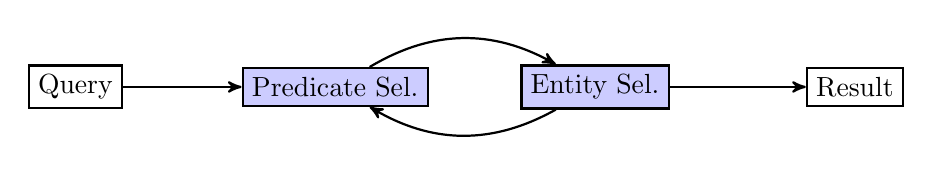
\begin{tikzpicture}[->,>=stealth',auto,node distance=3.3cm,
  thick,main node/.style={rectangle,draw, fill=blue!20},
  side node/.style={rectangle, draw}]
  \node[side node] (1) {Query};
  \node[main node] (2) [right of=1] {Predicate Sel.};
  \node[main node] (3) [right of=2] {Entity Sel.};
  \node[side node] (4) [right of=3] {Result};

  \path[every node/.style={font=\sffamily\small}]
    (1) edge node [right] {} (2)
    (2) edge [bend left] node [right] {} (3)
    (3) edge node [right] {} (4)
    (3) edge[bend left] node [left] {} (2);
%    (4) edge[bend right] node [left] {} (1);
\end{tikzpicture}
}
\end{frame}




%-------------------%
\section{Implementation}




\begin{frame}
  \tableofcontents[currentsection,hideallsubsections]
\end{frame}

%--------------------------%
\subsection{Predicate Selection}

\begin{frame}{Predicate Selection for predicate $p_{ij}$}

\begin{itemize}
\item<1-> The system presents a set of candidate predicates that match the given relation keywords $R_{ij}$
\item<2-> User is expected to select of subset of these predicates that align with her intent
\end{itemize}

\vspace{11pt}

\visible<3->{To be ensured that a small enough, yet accurate enough set of candidate predicates is presented to the user, in order to minimize user effort.}

\vspace{11pt}

\visible<4->{Predicate selection for $p_{ij}$, is performed for each of the relations $x_i \sim x_j$ specified initially by the user.}

\end{frame}



%-------------------%
\begin{frame}{Scoring candidate predicates}
\begin{align}
\text{Score}(p|\vec{q})& \propto \psi(p) \cdot \psi(R_{ij},p) \cdot \sum_{t_i,t_j,e_i,e_j} \phi_2(p, R_{ij}, C_i, C_j, K_i, K_j, t_i, t_j, e_i, e_j) \nonumber
\end{align}

where $\phi_2$ is defined as,
\begin{align}
\phi_2 =  \psi(t_i,t_j,p) \cdot \psi(C_i,t_i) \cdot \psi(C_j,t_j) \cdot \psi(e_i,e_j,t_i,t_j,p) \cdot \psi(K_i,e_i) \cdot \psi(K_j,e_j) \label{eq:phi2}
\nonumber
\end{align}

\end{frame}
%-------------------%

\begin{frame}{Computing $\psi(p)$}
\begin{itemize}
\item Compute frequency of occurrence of each predicate in one pass of the freebase triple dump.
\item The restricted freebase subset used for our experiments consists of \textbf{6,106} predicates.
\item The sum of all frequencies, equals the number of triples in our restricted subset, and is found to be \textbf{827,615,838}.
\end{itemize}
For computing $\psi(p)$, we have:
$$\psi(p) = \frac{\text{freq}(p)}{827,615,838}$$
\end{frame}

%-------------------%

\begin{frame}{Distribution of $\text{freq}(p)$}

\begin{figure}[h!] \label{preddist}
\centering
\includegraphics[width=0.7\textwidth]{./images/pred-freq}
\caption{Frequency distribution of Freebase predicates. Note that the scale on Y-axis is logarithmic.}
\end{figure}

\end{frame}

%-------------------%
\begin{frame}{Computing $\psi(R_{ij},p)$ - Using Lucene/Solr}
\begin{block}{}
The potential $\psi(R_{ij},p)$ denotes the compatibility between the relation keywords $R_{ij}$ and the freebase predicate $p$.
\end{block}

Construct micro-documents for each of the 6,106 freebase predicates with the following contents:
\begin{enumerate}
\item Name of the freebase predicate. For example, for the freebase predicate \url{/people/person/employment_history} the phrase ``employment history" is retained in the micro-document.
\item Synonyms of the freebase predicate name. WordNet is used to construct the list of synonyms. For example, the synonyms for ``spouse" are: \{``partner", ``married\_person", ``mate", ``better\_half"\}
.\end{enumerate}

\end{frame}

%-------------------%
\begin{frame}
Lucene implements a variant of the TfIdf scoring model. The Lucene scores are returned along with the top-$k$ search results--which may be directly used as a proxy for $\psi(R_{ij}, p)$.
\end{frame}

%-------------------%
\begin{frame}{Computing $\psi(R_{ij},p)$ - Pattern-based approach}
\begin{block}{}
ClueWeb09: Text corpus labeled with freebase entities.
\end{block}

\begin{itemize}
\item For each triple instance of each predicate, locate all corpus sentences that mentioned both participating entities.
\item Make the assumption that if $<e_1, p, e_2>$ is a triple and $e_1, e_2$ co-occur in a sentence, then this sentence is an evidence of the predicate relationship.
\item Each such sentence is parsed to obtain a dependency graph using the Malt Parser.
\item Words in the path connecting the entities are joined together and added to a candidate phrase dictionary, provided the path is at most three hops.
\end{itemize}

\end{frame}

%-------------------%
\begin{frame}{Computing $\psi(R_{ij},p)$ - Pattern-based approach}

Finally, the potential $\psi(R_{ij}, p)$ is computed as:
$$\psi(R_{ij},p) = \frac{n(p, R_{ij})}{\sum_{R'}{n(p, R')}}$$
where $R'$ ranges over all phrases that are known to
hint at $p$, and $n(p, R')$ denotes the number of sentences
where the phrase $R'$ occurred in the dependency
path between the entities participating in relation
$p$.

\begin{itemize}
\item Model is simplistic but ideal for freebase-scale data.
\item Noise in scores mitigated by collective scoring of predicates.
\end{itemize}
\end{frame}

%-------------------%

\begin{frame}{Pattern-based approach -- issues}

\begin{itemize}
\item Sparsity of corpus annotations or the rarity of Freebase triples in ClueWeb09.
\item E.g., for the Freebase relation \url{/people/person/profession}, very few annotated sentences are to be found.

\end{itemize}
One way to address this problem is to utilize relation type names in Freebase to map hints to relation types. Thus, in addition to the corpus-derived relation
model, we also use a language model that used Freebase relation type names as lemmas. E.g., the word `profession' would contribute to the relation type \url{/people/person/profession}.

\end{frame}

%-------------------%
\begin{frame}{Example queries -- pattern-based approach}

\textbf{Query 1:} $R_{ij}$ = ``music genre"
\begin{longtable}{| p{.55\textwidth} | p{.35\textwidth} |}
\hline
\textbf{freebase predicate} & $\psi(\text{``music genre", p})$ \\ \hline \hline
\url{/music/genre/artists} & -15.099850431212927 \\ \hline
\url{/book/magazine/genre} & -20.497121155364283 \\ \hline
\url{/computer/software/software_genre} & -22.372291455561907 \\ \hline
\url{/music/composition/place_composed} & -22.950699521833275 \\ \hline
\url{/music/artist/track} & -23.0148181515611 \\ \hline
\url{/music/composition/recordings} & -23.23339044018303 \\ \hline
\url{/user/ramanan/default_domain/musical_composer/musical_genre} & -25.10161835390006 \\ \hline
\url{/music/composer/compositions} & -25.72076068271463 \\ \hline
\url{/theater/play/productions} & -25.96101012469272 \\ \hline

\end{longtable}

\end{frame}
%-------------------%

\begin{frame}{Example queries -- pattern-based approach}

\textbf{Query 2:} $R_{ij}$ = ``company founder"
\begin{longtable}{| p{.55\textwidth} | p{.4\textwidth} |}
\hline
\textbf{freebase predicate} & $\psi(\text{``company founder", p})$ \\ \hline \hline
\url{/base/ballet/ballet_company/founder} & -13.436401752514346 \\ \hline
\url{/language/language_dialect/language} & -25.96800589848468 \\ \hline
\url{/sports/boxer/stance} & -27.002546059199332 \\ \hline
\url{/cvg/cvg_platform/games} & -27.009525090448083 \\ \hline
\url{/award/award_presenting_organization/award_categories_presented} & -27.059214681894424 \\ \hline
\url{/language/conlang/conlang_type} & -27.074404633446704 \\ \hline
\url{/business/business_location/parent_company} & -27.168006745432432 \\ \hline
\end{longtable}

\end{frame}


%-------------------%

\begin{frame}{Example queries for $R_{ij}$ -- Solr based approach}

\textbf{Query 1:} $R_{ij}$ = ``music genre"
\begin{longtable}{| p{.55\textwidth} | p{.4\textwidth} |}
\hline
\textbf{freebase predicate} & $\psi(\text{``music genre", p})$ \\ \hline \hline
\url{/music/music_video_genre/music_videos_of_this_genre} & 3.995606 \\ \hline
\url{/music/music_video/music_video_genre} & 3.995606 \\ \hline
\url{/music/music_video_choreographer/music_videos_choreographed} & 1.8530477 \\ \hline
\url{/film/film/music} & 1.4824381 \\ \hline
\url{/music/music_video_director/music_videos_directed} & 1.4824381 \\ \hline
\url{/book/book/genre} & 1.4766241 \\ \hline
\url{/book/magazine/genre} & 1.4766241 \\ \hline
\url{/book/short_story/genre} & 1.4766241 \\ \hline
\end{longtable}

\end{frame}


%-------------------%

\begin{frame}{Example queries for $R_{ij}$ -- Solr based approach}

\textbf{Query 2:} $R_{ij}$ = ``company founder"
\begin{longtable}{| p{.55\textwidth} | p{.4\textwidth} |}
\hline
\textbf{freebase predicate} & $\psi(\text{``company founder", p})$ \\ \hline \hline
\url{/people/family/founder} & 1.8162646 \\ \hline
\url{/food/cheese/farm_company} & 1.2482804 \\ \hline
\url{/automotive/manufacturing_plant/company} & 1.2420233 \\ \hline
\url{/business/company_brand_relationship/company} & 1.2420233 \\ \hline
\url{/business/company_name_change/company} & 1.2420233 \\ \hline
\url{/business/company_product_line_relationship/company} & 1.2420233 \\ \hline
\url{/business/company_product_relationship/company} & 1.2420233 \\ \hline
\end{longtable}

\end{frame}


%-------------------%


\begin{frame}{Computing $\psi(R_{ij},p)$}
\textbf{Concluding Remarks}: Even though the pattern-based approach utilizing ClueWeb09 corpus seems superior to the naive Lucene-based search technique, in practice we observed the latter to be much lighter on resources (and thus, faster) without compromising a lot on the accuracy of scores.

\end{frame}
%-------------------%

\begin{frame}{Computing $\psi(C_i,t_i)$}
\begin{block}{}
The potential $\psi(C_i,t_i)$ captures the compatibility between the category keywords $C_i$ and the freebase type $t_i$.
\end{block}
Language model for freebase types:
\begin{itemize}
\item Each type is described by one or more phrases through the link \url{/common/topic/alias}.
\item  We collect these into a micro-document and use a standard Dirichlet-smoothed language model from IR.
\item Relation types provide additional clues to types of the endpoint entities:

\end{itemize}


\end{frame}

%-------------------%
\begin{frame}{Type Language Model}
\begin{itemize}
\item Freebase relation types have the form \url{/x/y/z}, where \url{x} is the domain of the relation, and \url{y} and \url{z} are string representations of the type of the entities participating in the relation.
\item E.g., the (directed) relation type \url{/location/country/capital} connects from from \url{/location/country} to \url{/location/citytown}.
\item Therefore, ``capital" can be added to the set of descriptive phrases of entity type \url{/location/citytown}.
\end{itemize}
\end{frame}

%-------------------%
\begin{frame}{Example queries -- Type language model}
\textbf{Query 1:} $C_i$ = ``tv show"
\begin{longtable}{| p{.4\textwidth} | p{.35\textwidth} |}
\hline
\textbf{freebase type} & $\psi(\text{``tv show"}, t_i)$ \\ \hline \hline

\url{/tv/tv_rating} & -10.378222006687027 \\ \hline
\url{/tv/tv_soundtrack} & -10.378222006687132 \\ \hline
\url{/tv/tv_crewmember} & -10.378222006687363 \\ \hline
\url{/tv/tv_genre} & -10.378222006687558 \\ \hline
\url{/tv/tv_subject} & -10.378222006687638 \\ \hline
\url{/tv/video_host} & -10.782944611064888 \\ \hline
\url{/tv/tv_director} & -10.976166624970492 \\ \hline
\url{/tv/tv_actor} & -10.976171517623627 \\ \hline
\url{/tv/tv_song} & -10.976210661821304 \\ \hline
\url{/tv/tv_producer} & -10.97622044869509 \\ \hline
\url{/tv/tv_network} & -10.976244917322859 \\ \hline
\url{/tv/tv_program} & -10.976333021455918 \\ \hline

\end{longtable}
\end{frame}

%-------------------%
\begin{frame}{}

\textbf{Query 2:} $C_{i}$ = ``politician"

\begin{longtable}{| p{.5\textwidth} | p{.3\textwidth} |}
\hline
\textbf{freebase type} & $\psi(\text{``politician"}, t_i)$ \\ \hline \hline

\url{/government/politician} & -1.2971579353363734 \\ \hline
\url{/base/cdnpolitics/politician} & -2.080027054477 \\ \hline
\url{/base/braziliangovt/politician} & -2.0800270544771795 \\ \hline
\url{/base/coronationofgeorgevi1937/british_politician_guests} & -2.41161001352015 \\ \hline
\url{/base/irishpoliticians/irish_politician} & -2.5139595884469133 \\ \hline
\url{/base/membersofdail/irish_politician} & -2.5139752092688834 \\ \hline
\url{/base/portuguesepoliticians/politicians_of_the_monarchy} & -2.729032987285807 \\ \hline

\end{longtable}

\end{frame}

%-------------------%
\begin{frame}{Computing $\psi(K_i, e_i)$}
Lucene-based search approach:

\begin{itemize}
\item The micro-document for an entity $e_i$ can utilize the freebase description available for that entity.
\item Most freebase entities are linked to their description via the predicate \url{/common/topic/description}.
\item In general, the description is available in a number of languages; we restrict ourselves only to the English-language description available for entities.
\end{itemize}

Lucene-scores returned by querying the Solr index with $K_i$ are used as a proxy for $\psi(K_i, e_i)$.
\end{frame}

%-------------------%
\begin{frame}{Computing $\psi(K_i, e_i)$}
Word Embeddings approach:

\begin{itemize}
\item Google has made available\footnote{Google Code Archive - word2vec. \\ URL: \url{code.google.com/archive/p/word2vec/}} pre-trained entity vectors with freebase naming.
\item The word2vec `distance' function can be called to return the freebase entities with the least cosine distance from the keyword query $K_i$ and the cosine distance itself can be used in lieu of $\psi(K_i,e_i)$.
\end{itemize}
\end{frame}

%-------------------%
\begin{frame}{Computing $\psi(t_i, t_j, p)$}
Recall that we defined, $$\psi(t_i, t_j, p) = \frac{n(p;t_i,t_j)}{n(p)}$$
where,
\begin{itemize}
\item $n(p;t_i,t_j)$ denotes the number of triples in freebase that contain the predicate $p$ and whose subject and object have the freebase types $t_i$ and $t_j$ respectively
\item $n(p)$ as before, denotes the number of freebase triples containing $p$ as the predicate.
\end{itemize}

\end{frame}

%-------------------%
\begin{frame}{Computing $\psi(t_i, t_j, p)$}

\begin{itemize}
\item Iterate over the freebase triples dump and create a new intermediate dump in which each of the subject and object are replaced by their respective freebase types.
\begin{itemize} \item To speed up this replacement pass, we were required to maintain an in-memory dictionary mapping each freebase entity to its freebase type.
\item In case the object part of the triple was not found to be a freebase url, we simply ignored the triple.
\end{itemize}

\item Perform an external merge-sort of the dump to cluster together the rows with same value of $(t_i,t_j,p)$.
\item A final pass computed the quantity $n(p;t_i,t_j)$ by counting the number of adjacent rows with the same value of $(t_i, t_j,p)$.

\end{itemize}

The final $n(p;t_i,t_j)$ values are stored in a PostgreSQL table, along with $n(p)$ values in another table. The two quantities are retrieved from PostgreSQL to compute $\psi(t_i,t_j,p)$ when required during query processing.

\end{frame}


%-------------------%
\begin{frame}{Score computation for predicate selection}

\begin{itemize}
\item Summation over ($t_i$, $t_j$, $e_i$, $e_j$) tuples is likely to be infeasible within reasonable expectations of query processing time.
\item For our prototype implementation, we drop the summation over $e_i$, $e_j$ by simply setting $\psi(e_i,e_j,t_i,	t_j,p) = 1$, $\psi(K_i,e_i) = 1$, and $\psi(K_j,e_j)$.
\end{itemize}

Our simplified scoring model for predicates is thus,
\begin{align}
\text{Score}(p|\vec{q}) \propto \psi(p) \cdot \psi(R_{ij},p) \cdot \sum_{t_i,t_j} \psi(C_i,t_i) \cdot \psi(C_j,t_j) \cdot \psi(t_i,t_j,p) \nonumber
\end{align}

\end{frame}

%-------------------%
\begin{frame}{Predicate selection}

We use Lucene scores as a proxy for $\psi(R_{ij}, p)$.
\begin{itemize}
\item An Apache Solr index is built on micro-documents (one for each freebase predicate) containing WordNet synsets of the freebase predicate name.
\item Relation keywords $R_{ij}$ are used to retrieve the top-100 freebase predicates along with their Lucene scores by querying the Solr index.
\end{itemize}


The type language model as discussed previously is used for $\psi(C_i,t_i)$:
\begin{itemize}
\item The language model for types is queried by $C_i$ and $C_j$ to return two list of candidate types (along with $\psi(C_i,t_i)$ scores) of the formal types $t_i$ and $t_j$.

\end{itemize}

\end{frame}

\begin{frame}{Predicate selection}
\begin{itemize}
\item Probe each combination of $(t_i,t_j,p)$  and fetch $\psi(t_i,t_j,p)$ using a PostgreSQL query.
\item The product $\psi(C_i,t_i) \cdot \psi(C_j,t_j) \cdot \psi(t_i,t_j,p)$ is  marginalized by summing over all candidate types for $t_i$ and $t_j$.

\item The list of predicate scores thus obtained is sorted, and the top-100 predicates are sent to the user for selection.
\item The user may select one or more of these predicates, thereby concluding one predicate selection step.
\end{itemize}
\end{frame}

%-------------------%
\begin{frame}{Entity Selection}
We make use of the selector keywords $K_i$ for producing a ranked list of entities for further selection by the user.

$ \psi(K_i,e_i)$ as previously described is used for producing the ranked list.

\begin{itemize}
\item Micro-documents containing freebase entity description and aliases are constructed.
\item Solr index built on these micro-documents is queried with $K_i$.
\item Score returned by Solr for ranked entities is used as $ \psi(K_i,e_i)$.
\end{itemize}
\end{frame}

%-------------------------%
\begin{frame}{Result of the query}

\begin{itemize}
\item Result graph is formed by joining the sets of selected entities and predicates.
\item Care is taken to  ensure that all edges of the result graph are evidenced as triples in the freebase dump.
\item Result graphs are ranked by graph score = product of scores of all entities and predicates in the graph.
\end{itemize}
\end{frame}


%-------------------------%
\section{Demo}
\begin{frame}{Demo}

%\begin{block}{}
\begin{center}
\huge Prototype Demonstration
\end{center}
%\end{block}
\end{frame}


%-------------------------%
\begin{frame}[plain,c]

\begin{center}
\Huge Thank you for listening!
\end{center}

\end{frame}


\end{document}
